\documentclass[
  % -- opções da classe memoir --
  12pt,				         % tamanho da fonte
  oneside,			       % para impressão apenas no recto. Oposto a twoside
  a4paper,			       % tamanho do papel. 
  % -- opções da classe abntex2 --
  %chapter=TITLE,		   % títulos de capítulos convertidos em letras maiúsculas
  %section=TITLE,		   % títulos de seções convertidos em letras maiúsculas
  %subsection=TITLE,	 % títulos de subseções convertidos em letras maiúsculas
  %subsubsection=TITLE % títulos de subsubseções convertidos em letras maiúsculas
  % -- opções do pacote babel --
  english,		       	 % idioma adicional para hifenização
  brazil,			      	 % o último idioma é o principal do documento
]{abntex2}


% ---
% Pacotes fundamentais 
% ---
\usepackage{lmodern}		        	% Usa a fonte Latin Modern
\usepackage[T1]{fontenc}      		% Selecao de codigos de fonte.
\usepackage[utf8]{inputenc}   		% Codificacao do documento (conversão automática dos acentos)
\usepackage{indentfirst}	      	% Indenta o primeiro parágrafo de cada seção.
\usepackage{color}				        % Controle das cores
\usepackage{graphicx}			        % Inclusão de gráficos
\usepackage{microtype} 			      % para melhorias de justificação
\usepackage{listings}
\usepackage{amsmath}
\usepackage{fancyhdr}

% \setlength{\cftsubsubsecindent}{0pt}% Remove indent for \subsubsection

% ---
% Pacotes adicionais, usados apenas no âmbito do Modelo Canônico do abnteX2
% ---
\usepackage{lipsum}				% para geração de dummy text
% ---
% Pacotes de citações
% ---
\usepackage[brazilian,hyperpageref]{backref}	 % Paginas com as citações na bibl
\usepackage[alf]{abntex2cite}                  % Citações padrão ABNT
% --- 
% CONFIGURAÇÕES DE PACOTES

% Configurações do pacote backref
% Usado sem a opção hyperpageref de backref
\renewcommand{\backrefpagesname}{Citado na(s) página(s):~}
% Texto padrão antes do número das páginas
\renewcommand{\backref}{}
% Define os textos da citação
\renewcommand*{\backrefalt}[4]{
	\ifcase #1 %
		Nenhuma citação no texto.%
	\or
		Citado na página #2.%
	\else
		Citado #1 vezes nas páginas #2.%
	\fi}%
% ---


% ---
% Configurações do pacote backref
% Usado sem a opção hyperpageref de backref
\renewcommand{\backrefpagesname}{Citado na(s) página(s):~}
% Texto padrão antes do número das páginas
\renewcommand{\backref}{}
% Define os textos da citação
\renewcommand*{\backrefalt}[4]{
	\ifcase #1 %
		Nenhuma citação no texto.%
	\or
		Citado na página #2.%
	\else
		Citado #1 vezes nas páginas #2.%
	\fi}%
% ---
% ---
% Definindo formatação para exibição de código
% ---
\definecolor{codegreen}{rgb}{0,0.6,0}
\definecolor{codegray}{rgb}{0.5,0.5,0.5}
\definecolor{codepurple}{rgb}{0.58,0,0.82}
\definecolor{backcolour}{gray}{0.6}

\lstdefinestyle{mystyle}{
    commentstyle=\color{codegreen},
    keywordstyle=\color{magenta},
    numberstyle=\tiny\color{codegray},
    stringstyle=\color{codepurple},
    basicstyle=\ttfamily\footnotesize,
    breakatwhitespace=false,
    breaklines=true,
    captionpos=b,
    keepspaces=true,
    numbers=left,
    numbersep=5pt,
    showspaces=false,
    showstringspaces=false,
    showtabs=false,
    tabsize=2
}
\lstset{
  style=mystyle,
}
% ---
% 
% ---
\graphicspath{{../images/}}
% O tamanho do parágrafo é dado por:
\setlength{\parindent}{1.3cm}
% ---
% 
% ---
% Controle do espaçamento entre um parágrafo e outro:
\setlength{\parskip}{0.2cm}  % tente também \onelineskip
% ---
% 
% ---
% Espaçamento simples
\SingleSpacing
% ---
% Informações de dados para CAPA
% ---
\titulo{Uma Introdução a Haskell}
\autor{Gustavo Lopes Rodrigues \and Lucas Santiago \and Pedro Souza \and Thiago Henriques}
\local{Belo Horizonte}
\data{2020}
\instituicao{%
  Pontifícia Universidade Católica Minas Gerais
  }
\tipotrabalho{Trabalho de LIP}
% ---
% 
% ---
% informações do PDF
\makeatletter
\hypersetup{
     	%pagebackref=true,
		pdftitle={\@title}, 
		pdfauthor={\@author},
    	pdfsubject={Trabalho de Linguagem de programação em LaTeX},
	    pdfcreator={GLR, LSO, PS, THN},
		pdfkeywords={abnt}{latex}{abntex}{abntex2}{Linguagem de programação}, 
		colorlinks=true,       		% false: boxed links; true: colored links
    	linkcolor=black,          	% color of internal links
    	citecolor=blue,        		% color of links to bibliography
    	filecolor=magenta,      		% color of file links
		urlcolor=blue,
		bookmarksdepth=4
}
\makeatother

\makeindex

% ---
% Iniciando efetivamente o documento
% ---
\begin{document} 

    % Fazer com que as secções sejão subcapitulos
    \renewcommand{\thesection}{\noindent\arabic{chapter}.\arabic{section}}. 
    % ---
    % Selecionando linguagem
    % ---
    \selectlanguage{brazil}
    % ---
    % Retira espaço extra obsoleto entre as frases.
    % ---
    \frenchspacing
    % ---
    % Imprimir a capa 
    % ---
    \imprimircapa
    % ---
    % Imprimir a tabela de conteúdos(Sumário)
    % ---
    \pdfbookmark[0]{\contentsname}{toc}
    \tableofcontents*
    \cleardoublepage
    % ---
    % PARTE TEXTUAL
    % ---
    \textual
    % ---
    % Criar nova página e então iniciar a escrita
    % ---
    \newpage
    \chapter*[Introdução]{Introdução}
    \addcontentsline{toc}{chapter}{Introdução}

    Em 1930, Alonzo Church , matemático estadunidense apresentou o Cálculo Lambda, como parte da investigação dos fundamentos da matemática. O Cálculo Lambda é um sistema que
    estuda funções recursivas computáveis, e foi utilizada como base para as teorias e fundamentos matemáticos por trás do paradigma da Programação Funcional. Ele também
    pode ser considerado a primeira linguagem programação funcional, todavia, não foi projetada para ser executada em computadores, sendo apenas um modelo que descreve relações entre funções
    simples, permitindo criar funções mais complexas.

    Com o passar dos anos, varias linguagens funcionais foram criadas, sendo alguns exemplos a linguagem LISP em 1955 e a ML no final da década de 70. Porém, não
    havia um padrão para as linguagens desse paradigma, e quando chegou a segunda metade da década de 80, havia uma necessidade para criar uma única linguagem, que englobasse
    as melhores práticas de projeto, além de implementar as técnicas funcionais que estavam em alta na época.

    Nesse contexto Haskell foi criado em 1987, por Peyton Jones e Paul Hudak. Sendo assim a The Yale Meeting foi a primeira reunião presencial , no qual foi decidido
    os principais objetivos que a linguagem proporcionaria, como também a escolha do nome. 
    Segue as metas estabelecidas na reunião:

    \begin{itemize}
      \item Ser viável para o ensino, pesquisa e aplicações, incluindo sistema de larga escala;
      \item Ser completamente descritiva via publicação no tocante à sua sintaxe e sua semântica;
      \item Não ser proprietária, tal que qualquer um pudesse implementá-la e distribuí-la;
      \item Basear-se em ideias que envolvessem o senso comum;
      \item Reduzir a diversidade desnecessária de outras linguagens funcionais.
    \end{itemize} 

    A implementação de Haskell começou do zero, desenvolvendo funções únicas e tendo inspiração na linguagem Miranda que estava desempenhando um papel 
    importante na época. Em geral, essa linguagem passou por algumas versões que ajudou muito no desempenho e na adição de novas funções. 

    \newpage
    \chapter{Histórico sobre a linguagem, com sua cronologia}

    Depois desse evento, outras reuniões se sucederam e sendo assim no dia 01/04/1990, foi publicado primeiro relatório
    da versão 1.0 do Haskell. Durante os proximos 15 anos, Haskell teve o lançamento de diferentes versões, tranzendo outras
    funcionalidades para linguagem, entre elas se encontra Haskell'98 e Haskell 2010 que é a versão mais recente de Haskell.  

    O relatório da versão do Haskell'98 foi lançado em fevereiro de 1999. Ela surgiu no intuito de estabeler uma versão mais estável, 
    para ser possível realizar a documentação mais profunda da lingua em livros, já que o Haskell estava evoluindo muito rápido e ganhando 
    notoriedade.

    Em 2006 a equipe começou a planejar revisões anuais para adicionar o progresso do desenvolvimento da linguagem. Sendo assim a primeira revisão,
    publicada em julho de 2010, foi nomeada Haskell 2010 e nela foi incrementada uma serie recursos que antes não estavam disponiveis.
    Segue abaixo uma serie dos recursos que foram disponibilizados:
    
    \begin{itemize}
      \item Do and If Then Else 
      \item Hierarchical Modules
      \item Empty Data Declarations
      \item Fixity Resolution 
      \item Foreign Function Interface
      \item Line Comment Syntax
      \item Pattern Guards
      \item Relaxed Dependency Analysis
      \item Language Pragma
      \item Remove n+k patterns
    \end{itemize}

    Atualmente existem 3930 programadores com contas registradas que utilizam Haskell, sendo que 2566
    dessas contas são publicas e 1364 privadas. Por causa do número de programadores existem muitas 
    oportunidades nessa área, fazendo os empregos terem um sálario médio de \$80K à \$160K.

    Por mais que Haskell não seja tão utilizado como antes, muitos aplicações foram feitas com a linguagem. 
    Algumas aplicações são:

    \begin{itemize}
      \item A biblioteca open-source Semantic, implementada pelo GitHub, foi puramente escrito em Haskell.
      \item O Facebook implementa programas anti spam que são escritos e Haskell e são de código aberto.
      \item O Snap e Yesod, ambos frameworks para aplicações na web, foram feitos para suportar Haskell.
      \item O Linspire, sistema operacional comercial, tem Haskell como linguagem escolhida para o desenvolvimento das ferramentas no sistema.
      \item Xmonad, totalmente escrito em Haskell, é um gerenciador de janela para o sistema X Window System
    \end{itemize}

    \begin{figure}[ht]
      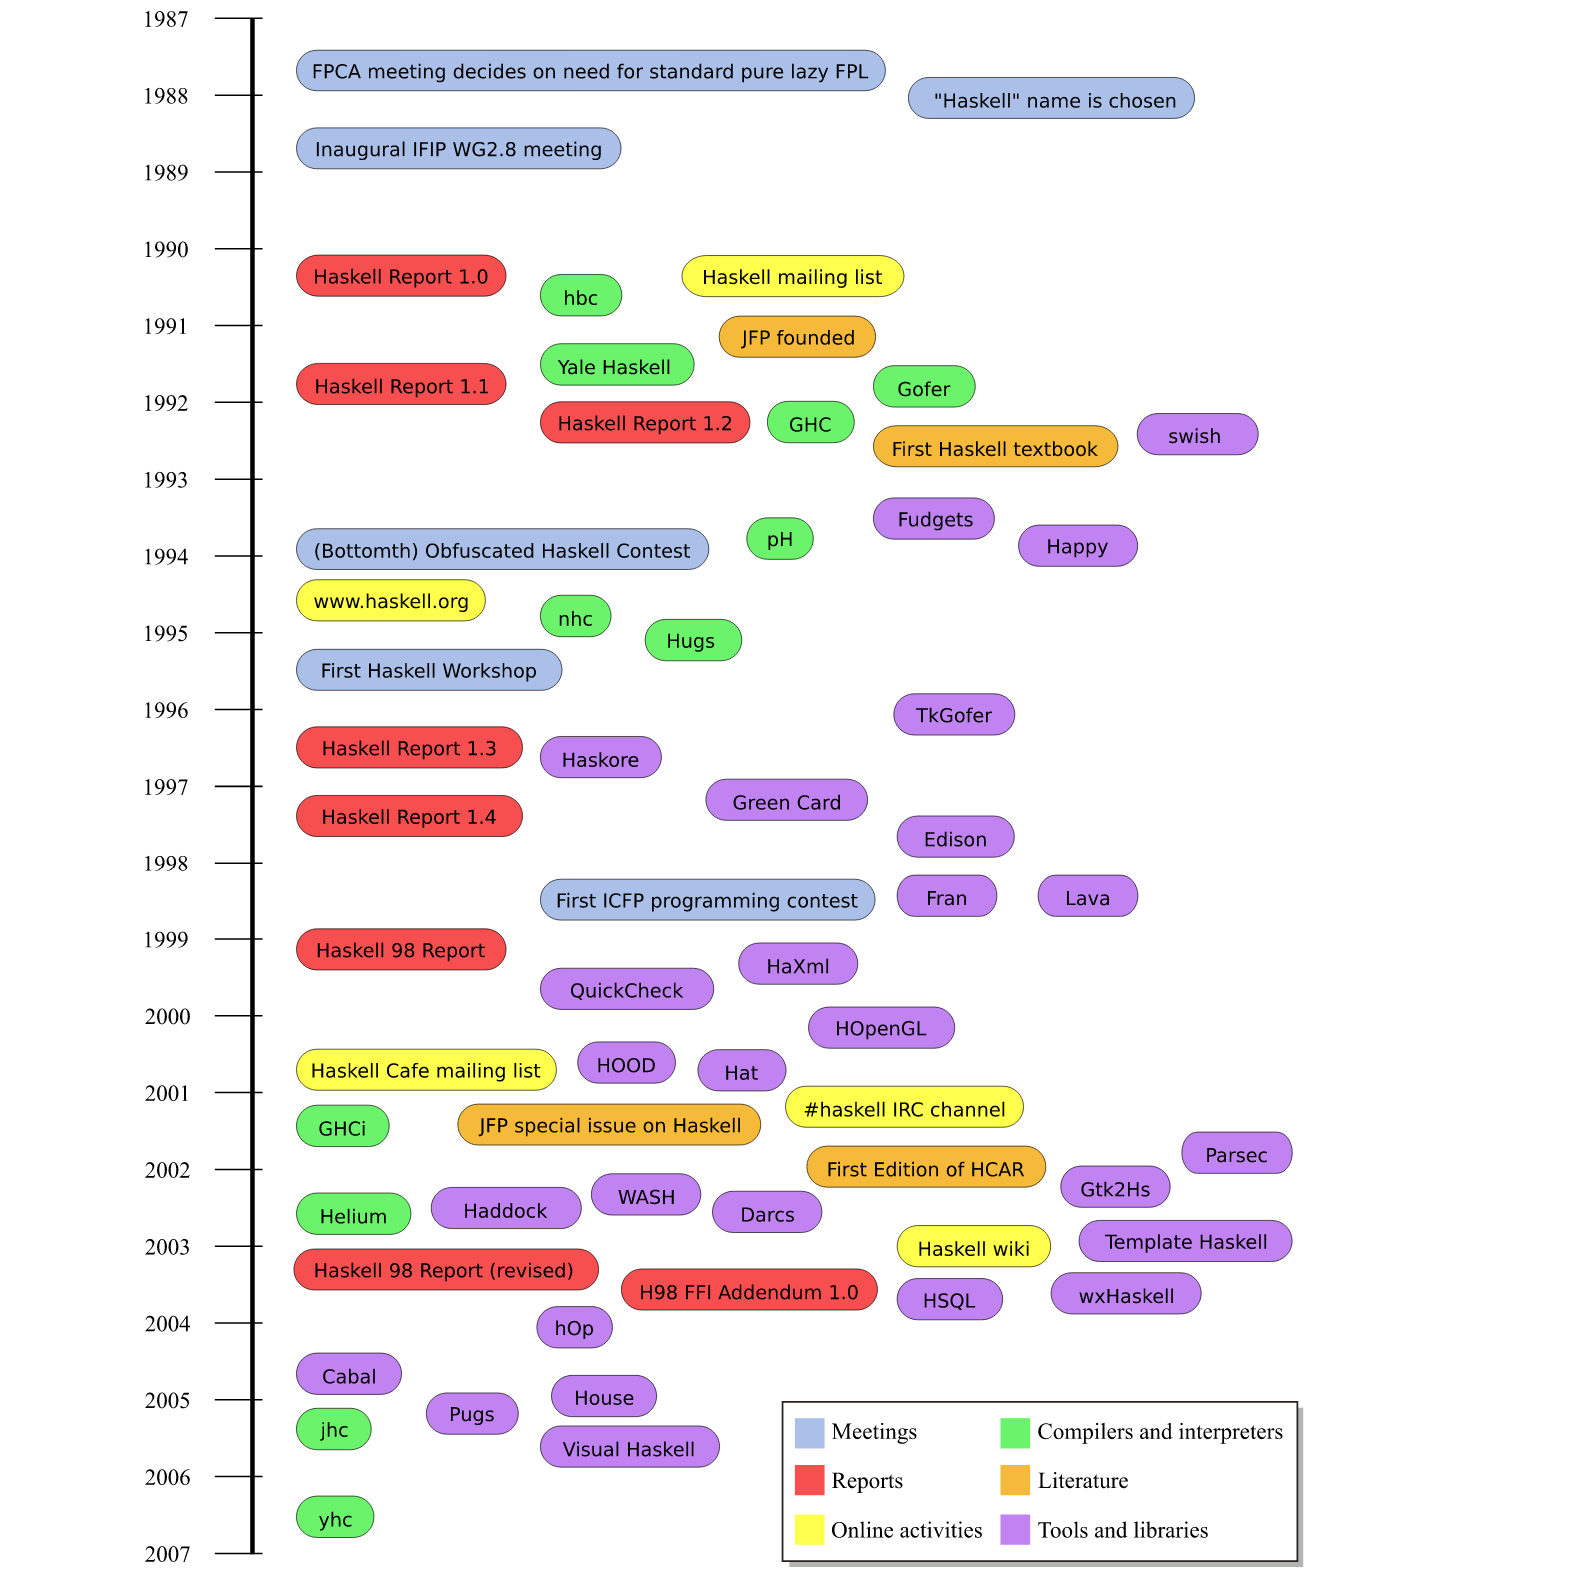
\includegraphics[width =\textwidth]{timeline.png}
      \caption{Cronologia do Haskell}
    \end{figure}

    \newpage

    \chapter{Paradigma a que pertence}

    O paradigma oferece e determina a visão que o programador possui sobre a estruturação
    e a execução do programa. Um exemplo bem famoso de paradigma é o POO (Programação orientada a objetos),
    conhecido por ser o modelo para linguagens como C++ e Java.

    Já a Programação funcional em espécifico, é um paradigma que descreve uma expressão matemática a ser avaliada,
    mapeando dos valores de entradas nos valores de retorno, por meio de funções. Em outras palavras: 
    a programação funcional é baseado em cima de funções que rodam no topo de outras funções. Programação 
    funcional está englobada junto ao grupo da Programação descritiva

    Eis mais algumas características deste paradigma

    \section{Dados imutáveis} 

    É possível declarar valores a variáveis, mas não pode mudar o valor dessas 
    delas durante a compilação. Isso acontece porque, diferente de linguagens imperativas(Como C), onde você
    atribui um valor e pode mudá-lo em execuções, variáveis em Haskell(por exemplo) possuem tipagem forte, logo 
    não sofrem efeitos colaterais(\emph{side effects}).

    \section{Funções puras}

    Também presentes em linguagens como JavaScript e Python, Funções puras são aquelas que recebem 
    um parâmetro \'input\' e sempre vão retornar o mesmo \'input\' sem causar efeitos colatreis
    ao programa.

    Este tipo de função é muito boa pelos seguintes aspectos
    
    \begin{itemize}
      \item facilita execução de códigos em paralelo, pois não impactam outras funcionalidades que estão em atuação
      \item Maior facilidade em criar cache, já que os mesmos parâmetros são sempre esperados.
    \end{itemize} 

    \newpage

    \section{Cálculo Lambda}
    
    Como mencionado anteriormente, o Cálculo Lambda está presente na programação funcional, e em Haskell não é diferente.
    Em Haskell, é possível utilizar as chamadas \emph{Expressões lambda} que são funções anônimas(sem nome), formadas por 
    uma sequência de padrões:

    \begin{itemize}
      \item Argumentos da função 
      \item Corpo
    \end{itemize}

    \begin{gather*}
      \text{Função anônima para calcular o dobro de x} \\ x \rightarrow x + x 
    \end{gather*}

    \section{Análise crítica} 

    As linguas que seguem o paradigma funcional se caracterizam em criar 
    funcionalidade dentro de estruturas de fácil compreensão e definição. Isso ajuda a manter 
    a fiabilidade, e leitura do código, principalmente quando integrado a forte tipagem. Além disso,
    táis códigos se caracterizam pelo alto nível de abstração, principalmente ao utilizar as funções,
    já que isso permite supressão de detalhes da programação, e garante uma menor probabilidade 
    de erros.

    Em contraste, tais ideias podem se tornarem complicadas, quando utilizadas dentro de contextos
    onde é necessário de muitas variáveis(Exemplo: Banco de Dados). Além disso, por conta que as funções 
    possuem a característica de serem recursivas por padrão, elas tendem a ser mais ineficientes no sentido
    computacionalmente, quando comparado as linguagens imperativas. Ainda nesse ponto, funções recursivas podem gerar maior uso de memória.

    %% Referencias dessa parte

    \nocite{haskellslides}
    \nocite{funcoespura}
    \nocite{funcoespura2}
    \nocite{haskellwikipedia}
    \nocite{abntex2-wiki-como-customizar}

    %%

    \newpage

    \chapter{Características mais marcantes da linguagem}

    A linguagem Haskell pode nos apresentar características peculiares que a destaca, entre elas o Lazy Evaluatio ou também conhecido como 'laziness'. Como exemplo,
    se ecrevermos um pequeno filtro ou parser em Haskell, não é necessário preocupar com os detalhes de ler input linha-por-linha ou bloco-por-bloco porque é possível
    simplesmente utilizar 'getContents' e então encadear uma série de funções. Uma vez que se tenha o 'laziness' na entrada, se tem o 'laziness' na saída porque imprimir
    algo não requer que tudo seja processado de uma só vez. Sendo assim, o programa fica com um design muito simples pois não é preciso lidar com buffers ou iterar sobre
    as linhas e ainda roda em um espaço constante.

    Além da técnica descrita acima, Haskell também apresenta benefícios em termos de expressividade, alcançado por 'matching the patterns' e o fato de que funções podem
    expressar coisas de forma sucinta mas legível, tornando mais fácil representar um problema e então, pensar na lógica, que é claramente identificável. Com Haskell,
    manipula-se funções tão fácil quanto a linguagem Pear manipula strings.

    A linguagem Haskell, assim como todas as outras linguagens, tem suas sintaxes e estruturação próprias. O centro da organização de um programa, seja ele feito em Haskell ou não,
    está definido nas funções que são criadas, porém, existem outros fatores importantes a serem observados.
    Nas primeiras linhas do programa são descritos os módulos que serão utilizados pelo mesmo. Para utilizar um módulo dentro de um programa basta colocar a seguinte declaração:

    \begin{gather*}
      import<nomeDoMódulo> as <nomeEspecifico> \\
      \text{Como importar módulos}
    \end{gather*}

    Já a criação de módulos é diferente, o cabeçalho deve ser escrito da seguinte forma:

    \begin{gather*}
      module<nomeDoMódulo>where \\
      <import<nomeDoMódulo> \\
      <declaraçãoDasFunçõesAseremExportadas> \\
      <declaraçãoDasVariáveisAseremExportadas> \\
      corpoDoMódulo \\
      \text{Cabeçalho de um módulo}
    \end{gather*}

    \newpage 

    Podemos importar outros módulos dentro de um módulo que estamos criando. O corpo do módulo é onde estão as funções criadas para serem utilizadas. Mesmo podendo haver vários módulos
    dentro de um mesmo arquivo, não é recomendado.
    Dentro da linguagem Haskell temos vários tipos de dados primitivos, operadores lógicos e e alguns caracteres especiais. Quanto aos operadores lógicos, os mais comuns são:
    \&\&, || e not. Para os tipos de dados primitivos, temos: Bool, Int, Char, String, Float e Double - tipos comuns da maioria das linguagens de programação. 
    Além dos operadores lógicos, Haskell proporciona os operadores aritméticos:

    \begin{table}[ht]
      \centering
      \begin{tabular}{|c | c |}
        \hline 
        + & Soma \\
        \hline 
        - & Subtração \\
        \hline 
        * & Multiplicação \\ 
        \hline 
        ${\wedge}$ & Potência \\ 
        \hline 
        div & Divisão inteira \\
        \hline 
        mod & Resto de divisão \\ 
        \hline 
        abs & Valor absoluto de um inteiro \\
        \hline 
        negate & Troca o sinal do valor \\
        \hline 
      \end{tabular}
      \caption{Operadores aritméticos}
    \end{table}

    Para finalizar os tipos primitivos em Haskell, os caracteres especiais possuem as seguintes representações:
    
    \begin{table}[ht]
      \centering
      \begin{tabular}{|c | c |}
        \hline 
        '\symbol{92}t' & Marca de tabulação \\
        \hline 
        '\symbol{92}n' & Nova linhas \\
        \hline 
        '\symbol{92}\symbol{92}' & Barra invertida \\ 
        \hline 
        '\symbol{92}'' & Aspas simples \\ 
        \hline 
        '\symbol{92}''' & Aspas duplas \\
        \hline 
      \end{tabular}
      \caption{Caracteres especiais}
    \end{table}

    Em Haskell, é possível criar tipos abstratos de dados, como tuplas e listas. Em uma tupla, podemos inserir um número determinado de dados com tipos predefinidos, já em uma lista os dados são
    todos do mesmo tipo (possibilitando a criação de uma lista que contenha tuplas, desde que os tipos de dados dentro das tuplas sejam iguais entre si). Apesar de serem tipos de dados abstratos,
    tuplas e listas não são as únicas dentro da linguagem, Haskell nos permite criar classes dentro dele.
    As classes em Haskell, são semelhantes às classes na orientação de objetos, com algumas implementações diferentes.
    Para começar uma classe, temos uma expressão como mostrada abaixo:
   
    \begin{gather*}
      class<nomeDaClasse><tipoDeEntrada>where<assinaturaDaClasse> \\
      \text{Definindo uma classe}
    \end{gather*}

    O nome da classe é um identificador e o tipo de entrada é para representar o tipo de dado, ou uma variável que atuaria como variável de tipo - possibilitando que a classe aceite qualquer tipo
    de dado na entrada. Sendo assim, o tipo de entrada pode ser tanto um inteiro, um char ou até uma string, dependendo da intenção do usuário.

    Por fim, não podemos deixar de falar no tratamento de exceção em Haskell, que é feito, não surpreendentemente, por meio de expressões. O comando catch é uma função cujo primeiro parâmetro
    uma expressão a executar e o segundo parâmetro é o que deve ser feito caso ocorra uma exceção. Além do comando catch, temos as palavras chaves raise e throw, que são utilizadas para definirmos
    exceções definidas e especificadas pelo programador.

    \begin{itemize}
      \item Como dito anteriormente, a linguagem só faz utilização de funções e funções dentro de funções. Por isso
      Haskell é descrito como puramente funcional.
      \item Haskell possui uma sintaxe simples, elegante e concisa. Como resultado, programas em Haskell possuem 
      poucas linhas. 
      \item Além disso, a linguagem usa avaliação preguiçosa(Lazy evaluation), que é uma técnica para atrasar a computação 
      até um ponto em que o resultado da computação é considerado necessário.
      \item Tipagem estática: Verificação dos tipos usados em dados e variáveis para 
      garantir que sempre está sendo usado um tipo que é esperado em todas as situações. 
      \item Função de ordem superior: Função que tem como argumento uma outra função, ou que produz 
      uma função como resultado.
      \item Antes da execução de um programa, os compiladores e interpretadores realizam uma checagem forte de tipos
      de dados, verificação monomórfica e verificação polimórfica.
    \end{itemize}

    \newpage

    \chapter{Linguagem similares ou confrontantes}

    \begin{itemize}
      \item Prolog
      \item LISP 
      \item Scheme 
      \item ML 
      \item Miranda 
      \item Elixir 
    \end{itemize}

    \newpage

    \chapter{Exemplo(s) de programa(s)}

      \setcounter{section}{0}

      \section{Hello World em Haskell}
      \lstinputlisting[language=haskell]{helloworld.hs}

      \section{Quicksort}
      \subsection{Exemplo de Quicksort em C}

      \lstinputlisting[language=c]{quicksort.c}
      \subsection{Exemplo de Quicksort em Haskell usando compreensão de lista} 

      \lstinputlisting[language=haskell]{quicksort_list.hs}      

      \newpage

      \subsection{Exemplo de Quicksort em Haskell usando a função filter}

      \lstinputlisting[language=haskell]{quicksort_filter.hs}

      \section{Explicação dos algoritmos}
      Os algoritmos em Haskell são extremamente compactos em relação à C. Sua sintaxe não tem foco
      em programar diretamente a memória, como acontece em C. Começando pelo \emph{Hello World} simples que possui ou evoluindo
      para um quicksort, a lingua mostra-se bem compacta e direta na resolução do problema.

      No primeiro exemplo, foi usado \emph{list comprehension} para resolver o problema. Na primeira linha,
      foi declarado uma lista vazia, mas poderia ser uma lista contendo quaisquer valores. A segunda linha
      cria uma função recursiva e 

      \subsection{Exemplo de Quicksort em Haskell usando a função filter}

      \lstinputlisting[language=haskell]{quicksort_c2haskell.hs}

      \newpage

      \subsection{Exemplo de Quicksort em Haskell usando a função filter} 

      \lstinputlisting[language=haskell]{quicksort_c2Haskellresumido.hs}

      \nocite{beginnersbook}

    \newpage

    \phantompart

    \chapter*[Considerações finais]{Considerações finais}
    \addcontentsline{toc}{chapter}{Considerações finais}

    Após trabalhar nessa linguagem por quase um mês, ficou claro para toda a equipe que Haskell é uma linguagem diferenciada. Possui
    uma história que foi essencial para sua formação, sem esquecer, é claro, que foi uma língua desenvolvida de forma comunitária.
    Há grandes obstáculos em ingressar nessa língua, principalmente por documentação excassa e a documentação oficial em maioria ser
    paga ou extremamente complexa para iniciantes. 
    
    Por muito tempo, Haskell não foi uma língua unificada, cada pessoa que entrava no projeto criava uma versão diferente sem que um líder
    principal coordenasse como ela estava evoluindo. Falta de uma unidade atrasou um pouco a língua ser adotada pela comunidade.
    Por conta da falta de uma documentação única, a dificuldade de aprendizado foi outro grande ponto negativo que impactou diretamente
    na falta de profissionais que a utilização, ficando apenas fechada em um ambiente científico como universidades.

    Entretanto depois de tudo que vimos, a linguagem se apresenta de forma bem mais positiva do que todas essas ideias
    citadas acima. Ela apresenta vários recursivos interessantes, como cálculos lambda, recursões simples e amarrações de funções
    em variáveis de forma simples. Há vários tutoriais distribuidos pela internet. Mesmo que
    poucas pessoas programem nessa língua, possui uma comunidade bem forte que a mantém.

    Por fim, o grupo entendeu que Haskell desempenhou seu papel na história da computação. Além disso,
    várias empresas ainda o adotam por entenderem a importância de seu uso, feito para cálculos científicos e precisos.
    Ainda dentro do contexto de programação funcional e uso de cálculos lambda, Haskell ainda é uma, se não a melhor,
    língua para ser utilizado.

    \newpage

    \postextual

    \bibliography{abntex2-modelo-references}
    \begin{apendicesenv}
      
        \partapendices

        %Corrigir erro da numeração dos apendices
        \setcounter{chapter}{0}
        \renewcommand{\thechapter}{\Alph{chapter}}%

        \chapter{Gustavo Lopes}

        O que eu achei de Haskell? Como um usuário de longa data de linguagens orientadas a objeto(OOP), 
        como Java, C++ e mais recentemente Dart, minha experiência inicial com Haskell foi...
        um pouco estranha. Fiquei muito curioso e até encucado em ver Haskell executar códigos, que em
        outras linguagens precisariam ocupar 50 linhas, em apenas 2 ou 3 linhas, como foi o Quicksort.

        Além disso, lendo sua história, achei extremamente fascinante toda a concepção do Haskell,
        mas fiquei até triste, vendo que é muito difícil encontrar muitas pessoas falando sobre essa linguagem, que nasceu 
        do esforço coletivo de vários programadores, mas que hoje não recebe tanto apoio como outras linguagens.

        Por fim, como curiosidade, eu estava procurando sobre como fazer interfaces em C++ quando
        descobri que a WxWidgets, uma biblioteca para criar interface cross-platform , também possui 
        sua versão para Haskell, chamada WxHaskell.

        \begin{figure}[ht]
          \includegraphics[width =\textwidth]{gebob.png}
          \caption{GeBoP, um jogo de tabuleiro feito em Haskell, usando WxHaskell}
        \end{figure}

        \newpage

        \chapter{Thiago Henriques}
        
        Bom, como posso expressar o que eu senti aprendendo sobre essa nova linguagem? Eu gosto muito das linguagens de alto nível, principalmente Python,
        então no começo devo admitir que senti uma certa um desafio. Porém sinto que Haskell conseguiu cumprir o 
        seu propósito e possibilitou a criação de novas.

        Em geral fiquei fascinado como a linguagem foi implementada e a tomada de decisão da equipe com o passar do tempo. A implementação
        possibilitou a adição de diversas funcionalidades únicas da linguagem e facilitou o desenvolvimento mais fluido da mesma.
        Além disso, achei interresante como em alguns códigos de Haskell eram necessário poucas linhas para se executar uma ação, assim
        me lembrando um pouco de Python.

        Eu observei que Haskell possui diversas implementações no mercado e muitos projetos de código aberto que utilizam da linguagem.
        Um dos projetos que eu achei muito interessante foi o Detexify, feito totalmente em Haskell, que tem como objetivo simplificar a 
        busca de simbolos especiais para aqueles que trabalham em Latex. O usuário só precisa desenhar o símbolo em uma caixa para mostrar 
        o comando do Latex.
        
        \begin{figure}[ht]
          \centering
          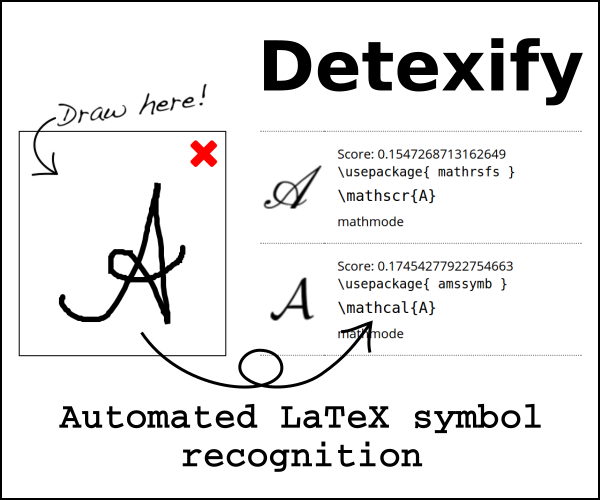
\includegraphics[scale=0.8]{detexify.png}
          \caption{Interface do Detexify}
        \end{figure}

        \newpage 

        \chapter{Lucas Santiago}

        Na minha opinião, Haskell se apresenta de uma forma muito diferente da maioria da outras línguas. 
        Parafraseando Fábio Akita: Cada língua de programação não é mais do que uma ferramenta
        para resolver um problema. 

        \begin{figure}[ht]
          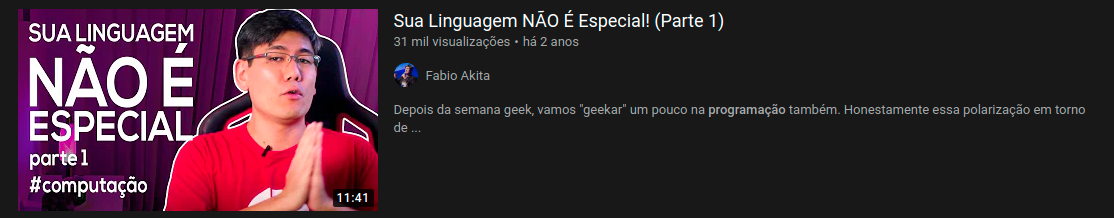
\includegraphics[width =\textwidth]{fabio_akita_lingua.png}
          \caption{\href{https://www.youtube.com/watch?v=p9-WuJbVHHc}{Fábio Akita explicando que linguas de programação são apenas feitas para resolver problemas!}}
        \end{figure}

        Os problemas que Haskell se propôs a resolver são cálculos matemáticos
        funcionais. O paradigma funcional dessa língua torna ela bem resistente a efeitos colaterais. Além de ser uma língua
        \emph{cross-platform}, extremamente importante para todas aquelas pessoas que precisem de uma língua que funcione
        em qualquer sistema operacional. 

        Como um programador de C/C++ e Python, vejo que Haskell está em um nível intermediário entre essas línguas.
        É interessante ver uma língua de alto nível com tipagem estática, torna o código bem estável - chances baixas de 
        resultar em erros -, tipagem é fundamental quando se quer garantir precisão de valores e tipos nos cálculos.

        Concluindo, não foi tão intuitivo aprender Haskell, ele possui várias propriedades que não existem em nenhuma das línguas
        que conhecia. Entretando, isso foi extremamente positivo para mim, aprendi várias coisas novas. Abaixo há
        mais um vídeo do Fábio Akita, dessa vez citando que nem sempre é fácil aprender algo novo. Em programação,
        quando você aprende da forma correta, várias novas possibilidades de resolução de problemas começam a aparecer.

        \begin{figure}[ht]
          \includegraphics[width =\textwidth]{fabio_akita_programar_eh_dificil.png}
          \caption{\href{https://www.youtube.com/watch?v=V7oUDL7E1g4}{Fábio Akita explicando que programação nem sempre é fácil.}}
        \end{figure}

        \newpage

        \chapter{Pedro Souza}

        Haskell definitivamente é uma linguagem um tanto quanto diferente das outras que são consideradas mais comuns, JAVA, C++, C\#, Javascript,
        PYTHON, etc. Apesar de não ter uma sintaxe muito complexa, sua implementação pode ser um pouco estranhada para quem está começando a conhecer
        a linguagem. 
    
        O fato de ser baseada em expressões, Haskell se torna um tanto quanto amedrontador para programadores novos, com pouca experiência e que estão
        mais acostumados com as linguagens mais usuais. Apesar de ter estudado e descoberto um pouco mais sobre a linguagem, admito que continuo 
        relutante quanto a usá-la. Talvez por ser um programador ainda em formação e com pouca experiência, não consigo ainda pensar em aplicações 
        que necessariamente teriam de ser feitas com Haskell.
    
        Como muitas outras linguagens por aí, Haskell continua muito oculta, sem muito reconhecimento e fama, um grande exemplo disso é que se pesquisarmos
        "Haskell" no google, encontraremos algum resultado sobre a linguagem apenas na segunda página e no último item encontrado. E aqui entre nós, quantas vezes vamos
        até a segunda página do google em alguma pesquisa?
    
        \begin{figure}[ht]
            \centering 
            \includegraphics[scale=0.3]{Haskellgoogle.png}
            \caption{Haskell, linguagem de programação apenas no último item da segunda página do google}
        \end{figure}

    \end{apendicesenv}

    \phantompart

    \printindex

\end{document}


